%File: datawiseagent_paper.tex
\documentclass[letterpaper]{article} % DO NOT CHANGE THIS
\usepackage{aaai24}  % DO NOT CHANGE THIS
\usepackage{times}  % DO NOT CHANGE THIS
\usepackage{helvet}  % DO NOT CHANGE THIS
\usepackage{courier}  % DO NOT CHANGE THIS
\usepackage[hyphens]{url}  % DO NOT CHANGE THIS
\usepackage{graphicx} % DO NOT CHANGE THIS
\urlstyle{rm} % DO NOT CHANGE THIS
\def\UrlFont{\rm}  % DO NOT CHANGE THIS
\usepackage{natbib}  % DO NOT CHANGE THIS AND DO NOT ADD ANY OPTIONS TO IT
\usepackage{caption} % DO NOT CHANGE THIS AND DO NOT ADD ANY OPTIONS TO IT
\frenchspacing  % DO NOT CHANGE THIS
\setlength{\pdfpagewidth}{8.5in} % DO NOT CHANGE THIS
\setlength{\pdfpageheight}{11in} % DO NOT CHANGE THIS
\usepackage{booktabs}
\usepackage{tabularx}
\usepackage{amsmath}
\usepackage{amssymb}
\usepackage{algorithm}
\usepackage{algorithmic}
\graphicspath{{figures/}{./}}
%
\pdfinfo{
/TemplateVersion (2024.1)
}

\setcounter{secnumdepth}{0}

\title{Toward Resource-Aware Data Science Agents: Task Adaptation, Structured Interaction, and Cost-Controlled Scheduling}

\author{
    Ziyi Ran\equalcontrib, Zhixiang Yu\equalcontrib, Heng Zhang\equalcontrib\\
}

\affiliations{}

\begin{document}

\maketitle

\begin{abstract}
Large language model (LLM)-based agents are increasingly used to automate data science workflows, yet practical deployment exposes three linked weaknesses: task-specific failure modes that generic pipelines do not address, long-context interactions that can degrade rather than improve answer quality, and high cost from using large models uniformly across all stages. We study these challenges through DatawiseAgent, a multi-stage agent framework evaluated on two complementary benchmarks: InfiAgentBench for closed-form data analysis and DataModeling for Kaggle-style predictive modeling. Our contributions are threefold. First, we introduce a task-aware harness that routes questions by concept, difficulty, and format requirements to protocol-specific constraints, improving medium-difficulty accuracy by 8.2 percentage points on InfiAgentBench and eliminating format-level answer extraction errors. Second, we design a structured interaction pipeline that decomposes notebook-style conversations into verifiable artifacts (DataCard, Answer Spec, Verifier, Final Block), enabling targeted retry on failure without re-feeding full conversation logs. Third, we propose EqTok, an equivalent-token resource metric based on API pricing ratios, together with a risk-stratified scheduler that assigns deterministic processing to low-risk stages and reserves stronger models for high-risk reasoning, achieving 40\% resource savings while maintaining 96\% of baseline accuracy. We also identify boundary conditions: training-free harness engineering cannot fully substitute for model capability on hard tasks, and uncurated memory degrades retrieval signal-to-noise ratio over time. These findings yield practical design principles for building cost-effective and reliable data science agents.
\end{abstract}

\section{Introduction}

The rapid advancement of large language models (LLMs) has catalyzed autonomous agents for data science tasks ranging from exploratory analysis to predictive modeling~\cite{wang2024data, guo2024data}. These agents typically operate in a notebook-style environment: they plan, generate code, execute analyses, and debug errors through a multi-turn interaction with the user or environment~\cite{infiagentbench, chen2021evaluating}. The promise is compelling: a single agent can ingest a CSV file, interpret a natural language question, produce executable analysis code, and return a verified answer without human intervention.

Despite strong demonstrations on curated benchmarks, deployment in cost-sensitive, multi-task settings reveals three under-explored tensions. \textbf{First}, failure modes are not uniform across tasks. On InfiAgentBench~\cite{infiagentbench}, failures often involve answer-name drift, statistical definition ambiguity, and output format instability: the agent may compute the correct statistic but render it under the wrong answer key or in an unparseable format. On DataModeling benchmarks derived from Kaggle competitions~\cite{kaggle}, failures instead involve structurally valid but information-poor submissions, such as constant predictions, collapsed multi-class outputs, and missing manifest files. A generic harness with identical constraints for every task cannot address this heterogeneity. \textbf{Second}, the common assumption that more interaction rounds yield better performance conflates structured verification with aimless dialogue. Long notebook histories increase the chance that stale variables, debug outputs, or earlier wrong answers contaminate the final response, consistent with the ``lost in the middle'' effect~\cite{liu2024lost}. Cost also grows with context length. \textbf{Third}, using large reasoning models uniformly across the pipeline inflates API cost without proportional accuracy gains. Many sub-tasks---data profiling, format validation, and answer rendering---are deterministic or require only lightweight instruction following, yet they are often billed like complex code generation.

In this paper, we present an end-to-end study of these three tensions through DatawiseAgent, a multi-stage agent framework evaluated on InfiAgentBench (257 data analysis questions across three sub-tasks: ABQ, PASQ, UASQ) and DataModeling (74 Kaggle competition tasks). Our key insight is that these three tensions are not independent---they jointly determine whether a deployed agent is simultaneously accurate, reliable, and affordable. We make the following contributions:

\begin{itemize}
    \item \textbf{Task-Aware Harness (Section~\ref{sec:task})}: We design a routing mechanism that classifies questions by difficulty, statistical concept, and expected output format, then dispatches each question type to a protocol-specific constraint pipeline (Answer Spec, Skill Checklist, Verifier). This eliminates format-level extraction errors and improves medium-difficulty ABQ by 8.2pp and hard-difficulty ABQ by 12.3pp on InfiAgentBench.
    \item \textbf{Structured Time-for-Performance (Section~\ref{sec:structured})}: We decompose long agent interactions into discrete, verifiable artifacts and enforce that retry operations only receive failure-point diagnostics rather than full conversation histories. We compare lightweight versus full semantic verification regimes and characterize when additional structure yields net benefit versus when it introduces unnecessary overhead.
    \item \textbf{Resource-Aware Scheduling (Section~\ref{sec:resource})}: We introduce EqTok, an equivalent-token metric based on API pricing ratios, and a risk-stratified scheduler that routes low-risk sub-tasks to deterministic programs or small instruct models while reserving large reasoning models for high-risk code generation and debugging. This achieves a 40\% EqTok reduction while retaining 96\% of baseline accuracy.
    \item \textbf{Boundary Characterization (Section~\ref{sec:discussion})}: We document failure regimes where training-free harness improvements are insufficient---hard multi-concept questions, low-information predictive submissions, and memory saturation---and derive design principles for future agent development.
\end{itemize}

\section{Related Work}

\subsection{LLM Agents for Data Science}

Recent work has demonstrated that LLMs can serve as the reasoning core of data science agents. Frameworks such as OpenHands~\cite{wang2024data} and Data Interpreter~\cite{guo2024data} orchestrate LLM calls within a structured environment to perform multi-step data analysis. These systems share a common pattern: the agent receives a natural language question and a dataset, plans a sequence of analysis steps, generates and executes Python code, and formats the final answer. AutoGen~\cite{wu2023autogen} introduces multi-agent conversation patterns, where specialized agents handle different aspects of the workflow. InfiAgentBench~\cite{infiagentbench} provides a standardized evaluation suite covering answer-book questions (ABQ), partially-assisted single questions (PASQ), and unassisted single questions (UASQ). Unlike these works, which focus on maximizing single-run accuracy, our study systematically examines the accuracy--cost--reliability trade-off across heterogeneous task distributions.

\subsection{Harness Design and Prompt Engineering}

The effectiveness of LLM agents depends critically on the ``harness''---the scaffolding of prompts, constraints, and validation rules surrounding the model~\cite{white2023prompt}. Prior work has explored constraint decoding~\cite{lu2024chameleon}, self-consistency verification~\cite{wang2022self}, and structured output parsing~\cite{zheng2023judgelm}. Chain-of-thought prompting~\cite{wei2022chain} and tree-of-thought reasoning~\cite{yao2023tree} improve reasoning quality through structured intermediate steps. However, most harness designs apply uniform constraints across all task types. Our work introduces task-specific routing, where the harness configuration is selected based on question taxonomy, and couples harness design with resource allocation.

\subsection{Resource-Efficient LLM Deployment}

The computational cost of deploying LLMs at scale has motivated research on model cascading~\cite{varshney2022model}, speculative decoding~\cite{leviathan2023fast}, and mixture-of-agents~\cite{wang2024mixture}. In the agent context, recent work has explored routing sub-tasks to smaller models~\cite{chen2024fusellm, ong2024route}. Our contribution extends this line by integrating task difficulty, verification feedback, and interaction history into a unified risk-stratified scheduler, and by proposing EqTok as a pricing-normalized resource metric that enables fair comparison across heterogeneous model families.

\subsection{Memory and Context Management in Agents}

Long-context LLMs enable agents to process extended interaction histories, but longer contexts do not monotonically improve performance~\cite{liu2024lost}. MemGPT~\cite{packer2023memgpt} introduces virtual memory management for LLM agents, with hierarchical storage and retrieval. Our work contributes empirical evidence from the data science domain: uncurated memory accumulation degrades retrieval quality, and we propose artifact-based communication with selective forgetting as a lightweight alternative that avoids the complexity of full virtual memory systems.

\section{Background: DatawiseAgent and Benchmark Analysis}
\label{sec:background}

\subsection{System Architecture}

DatawiseAgent consists of three layers. The \textbf{Agent Core} implements a finite-state transducer (FST) that transitions through four stages: (1) planning, which decomposes the question into analysis steps; (2) execution, which generates and runs Python code in notebook cells; (3) debugging, which diagnoses and fixes runtime or logic errors; and (4) post-debug filtering, which cleans up error cells and retains the working execution path. Each stage may trigger an LLM API call, with the default configuration using a single model for all stages regardless of difficulty.

The \textbf{Harness Layer} provides ten deterministic modules that wrap the agent core: DataCard (dataset schema profiling), Contract (answer specification), Skill Checklist (preprocessing requirements), Oracle (semantic verification rules), Verifier (post-execution constraint checking), Final Block (output formatting), Memory (interaction history storage), Search (multi-branch exploration), Recovery (error state recovery), and Rules (constraint definitions). These modules are all deterministic---they use pattern matching, regular expressions, and template rendering rather than LLM calls.

The \textbf{Evaluation Layer} manages benchmark execution, answer reformatting, closed-form scoring, and metric aggregation. It supports configurable ablation experiments where individual harness modules can be enabled or disabled.

Our experiments use Qwen model variants (8B, 14B, 32B, and 35B-A3B MoE) deployed via API, with Qwen3.5-35B-A3B serving as the strong reference and Qwen3.5-Flash serving as the weak-model testbed.

\subsection{Benchmark Profiles}

\textbf{InfiAgentBench (DA-Dev)} comprises 257 data analysis questions with the following distribution: Easy (82, 31.9\%), Medium (87, 33.9\%), Hard (88, 34.2\%). Each question provides a CSV dataset and a natural language query. Questions are annotated with data science concepts: Summary Statistics (90 questions), Correlation (58), Feature Engineering (37), Machine Learning (19), and Comprehensive Preprocessing (45). Notably, 107/257 (41.6\%) questions involve multiple concepts, with dual-concept combinations exhibiting the lowest accuracy (79.4\% vs.\ 90.7\% for single-concept). Questions span three sub-tasks: ABQ (answer-book questions with structured answer keys), PASQ (partially-assisted single questions), and UASQ (unassisted single questions). Evaluation uses exact-match accuracy (Q-Acc).

\textbf{DataModeling} comprises 74 Kaggle-style predictive modeling tasks spanning diverse domains. The agent must produce a valid CSV submission file and a manifest documenting model selection rationale. Evaluation uses completion rate (fraction of tasks yielding a parseable submission) and a normalized performance score aggregating domain-specific metrics (AUC, RMSE, log loss). The baseline Qwen2.5 achieves 68/74 completion with a performance score of 0.4290 at an average of 760.3 seconds per task.

\begin{figure}[t]
\centering
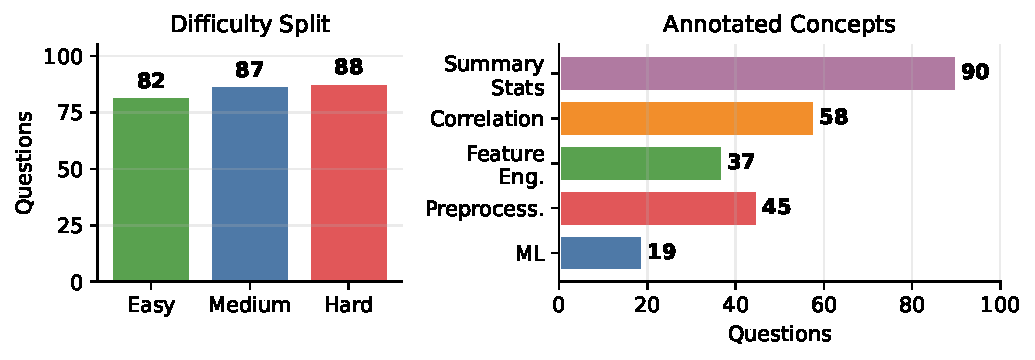
\includegraphics[width=\columnwidth]{task_profile}
\caption{InfiAgentBench profile used in our analysis. The split is balanced across difficulty levels, while concept labels concentrate in summary statistics, correlation, preprocessing, feature engineering, and machine learning.}
\label{fig:task_profile}
\end{figure}

\subsection{Failure Mode Taxonomy}

Systematic analysis of baseline results reveals distinct failure patterns per benchmark:

\textbf{InfiAgentBench failures} cluster around three categories: (1) \textit{answer-name mismatch}---the agent computes the correct statistic but assigns it to a differently named answer key in the final output; (2) \textit{statistical definition drift}---the agent misapplies filtering conditions, grouping variables, or rounding rules despite understanding the question intent; (3) \textit{format degradation}---the agent produces the correct value but renders it in an unparseable format such as a DataFrame or Series object instead of a scalar.

\textbf{DataModeling failures} cluster around: (1) \textit{low-information submissions}---constant predictions, single-class outputs for multi-class problems, or global-mean regression predictions; (2) \textit{manifest issues}---missing or incomplete documentation of model selection; (3) \textit{schema violations}---wrong column names, mismatched row counts, or incorrect ID columns.

\begin{table}[t]
\centering
\caption{Baseline performance on InfiAgentBench. Qwen3.5-35B-A3B serves as the strong reference. Qwen3-32B provides a comparable single-model baseline.}
\label{tab:baseline}
\begin{tabular}{lccc}
\toprule
\textbf{Setting} & \textbf{ABQ} & \textbf{PASQ} & \textbf{UASQ} \\
\midrule
Qwen3-32B (full) & 81.74\% & 86.21\% & 86.43\% \\
Qwen3.5-35B-A3B & 86.38\% & 90.16\% & 90.35\% \\
\bottomrule
\end{tabular}
\end{table}

These distinct failure patterns motivate our three-part optimization: task-specific routing addresses definition drift, structured interaction prevents context degradation, and resource-aware scheduling allocates model capacity where it matters most.

\section{Task-Specific Adaptation via Protocol Routing}
\label{sec:task}

\subsection{Task Router Design}

The central premise of the task-aware harness is that different question types require different constraint protocols. A Summary Statistics question needs strict enforcement of column selection and rounding precision; a Correlation question needs the method declared before computation; a Machine Learning question needs a model card rather than a fixed formula. Uniform constraints therefore either under-specify questions that need strict rules or over-specify questions that need modeling flexibility.

Figure~\ref{fig:da_hero_overview} summarizes the resulting DA-HERO pipeline. The task-aware routing block analyzes requirements and dispatches each question to a level-, concept-, and type-specific plan before execution; downstream verifier and finalizer modules then enforce the structured answer contract.

\begin{figure*}[t]
\centering
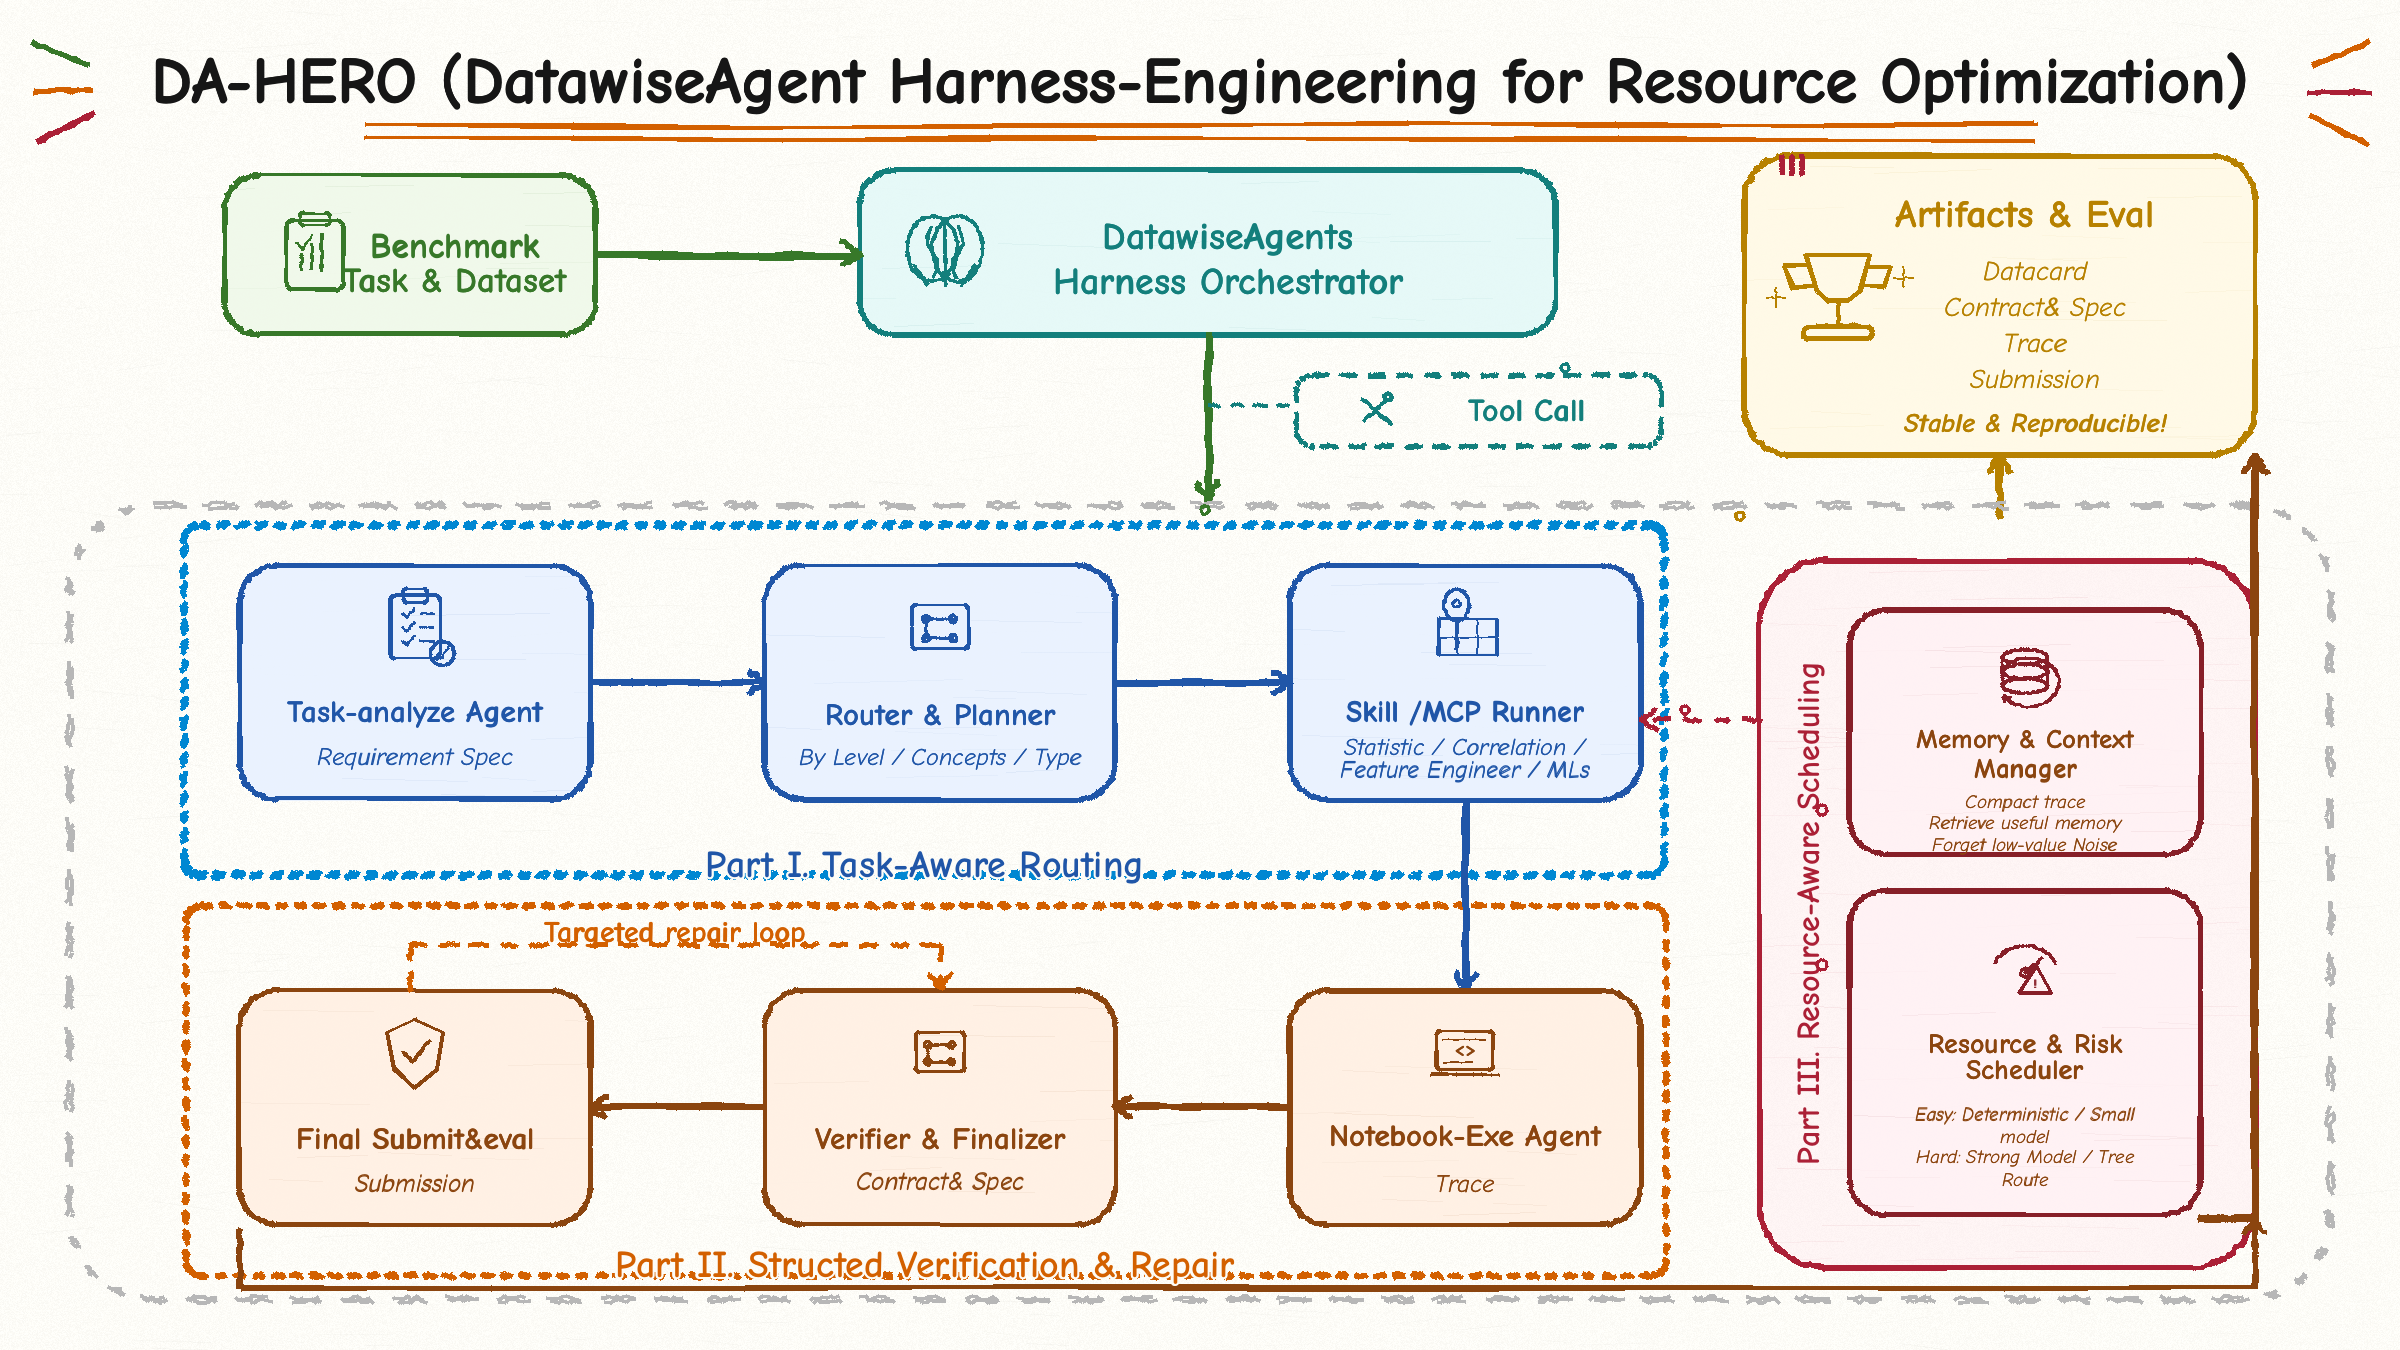
\includegraphics[width=0.96\textwidth]{2404.PNG}
\caption{DA-HERO overview for task-aware routing, structured verification, and resource-aware scheduling. The figure highlights how benchmark inputs are converted into requirement specifications, routed through concept-specific skills, checked by verifier/finalizer modules, and saved as reproducible artifacts.}
\label{fig:da_hero_overview}
\end{figure*}

We implement a \textbf{Task Router} that classifies each incoming question along four axes: (1) difficulty level (Easy/Medium/Hard), derived from benchmark metadata; (2) data science concepts (Summary Statistics, Correlation, Feature Engineering, Machine Learning, Comprehensive Preprocessing); (3) question-intent keywords (e.g., ``average,'' ``correlation,'' ``predict,'' ``transform''); and (4) expected output format (scalar, list, DataFrame, JSON).

Each question type maps to a \textbf{Harness Spec}, a protocol card specifying:

\begin{itemize}
    \item \textbf{Answer Spec}: the exact answer name, filtering conditions, grouping variables, statistical method, rounding precision, and explicitly forbidden operations (e.g., ``do not output a DataFrame'').
    \item \textbf{Skill Checklist}: the required preprocessing steps, ordered by dependency (e.g., ``check for missing values in column X before computing the mean'').
    \item \textbf{Output Contract}: the precise format template for the final answer block.
\end{itemize}

The router operates deterministically when benchmark metadata is available. In production settings without pre-annotated difficulty labels, it falls back to a lightweight 8B model for ambiguity resolution. After execution, a \textbf{Verifier} checks whether the output conforms to the Answer Spec before the Final Block renders it. The Final Block is deliberately deterministic rather than LLM-based: it extracts the verified answer value and wraps it in the required output format, eliminating format degradation as a separate failure mode.

\subsection{Task-Type-Specific Protocol Adjustments}

For \textbf{Summary Statistics} questions (90/257, the largest category), the harness enforces strict constraints on column selection, filtering order, and rounding precision. These questions have well-defined mathematical answers, so the harness can be maximally prescriptive. For \textbf{Correlation} questions (58/257), it requires the agent to explicitly declare the correlation method (Pearson, Spearman, Kendall) before computation and verifies that the declared method matches the computed result. For \textbf{Machine Learning} questions (19/257, all Hard), it requires a model card documenting algorithm choice, hyperparameters, and validation strategy, but the harness is less prescriptive about the modeling itself.

On the \textbf{DataModeling} side, we extend the harness with a \textbf{Quality Gate}: a submission validator that checks schema compliance (column names, row count, ID column), probability range (0--1 for classification tasks), and sample-level consistency with the test set. Submissions that pass structural validation but contain degenerate predictions (constant values, single-class outputs, global-mean regression) are flagged for repair. The Quality Gate also checks manifest completeness and flags missing documentation.

\subsection{Results on InfiAgentBench}

Table~\ref{tab:task_results} shows the impact of the task-aware harness. The harness rerender eliminates all format extraction errors---format error rate, reformat missing rate, and final block missing rate all drop to zero---and delivers consistent improvements across all sub-tasks and difficulty levels.

\begin{table*}[t]
\centering
\caption{Task-aware harness results on InfiAgentBench (Qwen3-32B). Bold indicates best per split.}
\label{tab:task_results}
\begin{tabular}{lcccc}
\toprule
\textbf{Setting} & \textbf{Split} & \textbf{ABQ} & \textbf{PASQ} & \textbf{UASQ} \\
\midrule
Baseline & Medium & 83.72\% & 86.19\% & 86.00\% \\
Harness rerender & Medium & \textbf{91.95\%} & \textbf{93.06\%} & \textbf{93.42\%} \\
\midrule
Baseline & Hard & 66.13\% & 78.49\% & 82.99\% \\
Harness rerender & Hard & \textbf{78.41\%} & \textbf{84.75\%} & \textbf{87.19\%} \\
\bottomrule
\end{tabular}
\end{table*}

\begin{figure*}[t]
\centering
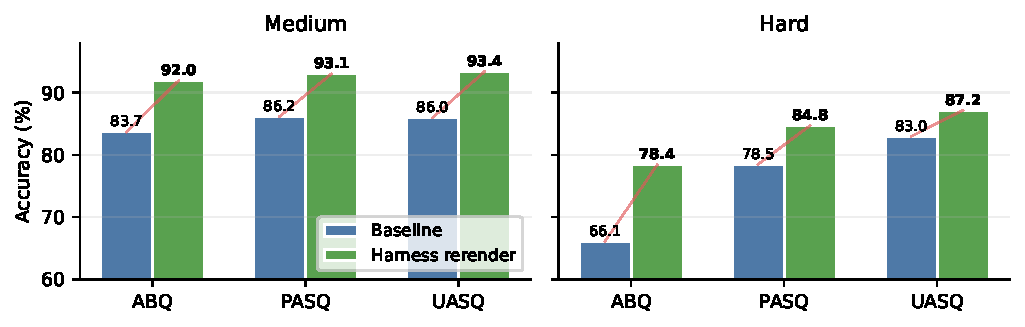
\includegraphics[width=0.86\textwidth]{task_harness_results}
\caption{Task-aware harness gains by split and sub-task. The largest absolute gain appears on Hard ABQ, where answer specification, verification, and deterministic final rendering prevent otherwise silent format and definition errors.}
\label{fig:task_harness_results}
\end{figure*}

On Medium questions, ABQ improves by 8.23 percentage points, demonstrating that format constraints and structured answer extraction directly eliminate preventable errors. The improvement on PASQ and UASQ (6.87pp and 7.42pp, respectively) confirms that answer specification benefits extend beyond format correction to statistical definition stabilization. On Hard questions, ABQ improves by 12.28 percentage points---the largest absolute gain---though the average number of execution branches rises from 1.0 to 2.97, indicating that the harness triggers additional exploration that increases search cost. This observation directly motivates our subsequent work on resource scheduling (Section~\ref{sec:resource}): more branches improve accuracy but must be managed to control cost.

\subsection{Results on DataModeling}

On DataModeling, Qwen3.5-35B-A3B achieves 73/74 completion with a normalized performance score of 0.5318 and an average time of 288.6 seconds, substantially outperforming the Qwen2.5 baseline (68/74, 0.4290, 760.3s). However, Qwen3-VL models (8B and 32B) achieve 74/74 structural completion while reaching performance scores of only 0.3127 and 0.2873, respectively. This exposes a critical \textbf{completion-to-performance gap}: structurally valid CSV files may still contain mean predictions, constant outputs, or missing manifests that escape basic format validation. Representative re-tests confirm the pattern. 8B Titanic (0.7877 AUC) and 32B Santander (0.8116 AUC) produce usable predictions for well-structured tabular tasks, but both require manifest repair and fail on tasks requiring domain-specific modeling strategies.

\section{Structured Time-for-Performance}
\label{sec:structured}

\subsection{The Problem with Unstructured Long Interactions}

Prior work often treats multi-turn interaction as a universal performance lever: the agent explores, errs, and self-corrects over dozens of notebook cells. Our analysis shows that this paradigm introduces three recurring failure modes:

\begin{enumerate}
    \item \textbf{Context Contamination}: As notebook history grows, the model increasingly confuses stale intermediate variables, debug outputs, and earlier incorrect answers with the final result. We observe cases where the agent correctly computes an answer in cell 5, debugs an unrelated error in cells 6--8, and then overwrites the correct answer with a debug intermediate in cell 9.
    \item \textbf{Non-Monotonic Harness Benefit}: Full semantic verification introduces communication overhead: the verifier's prompts consume context budget, and verification errors can block correct answers. In our experiments, full harness occasionally rejects correct answers due to overly strict oracle rules, particularly on questions where multiple valid statistical approaches exist.
    \item \textbf{Branch Proliferation Without Selection}: Multi-branch search increases the pool of candidate answers but does not inherently improve selection. Without a principled criterion for choosing among candidates, more branches can degrade performance by presenting the model with more alternatives to confuse.
\end{enumerate}

\subsection{Verifiable Artifact Pipeline}

We decompose the agent's interaction into six discrete stages, each producing a verifiable artifact that is independently checkable:

\begin{enumerate}
    \item \textbf{DataCard}: A deterministic profile of the dataset (column names, types, missing values, numeric ranges). Generated once by a program---not an LLM---and reused across all questions on the same dataset.
    \item \textbf{Answer Spec}: A structured specification extracted from the question text: answer name, required columns, filtering rules, aggregation method, precision, and output format. Parsed deterministically from question metadata when available; falls back to an 8B model for ambiguous questions.
    \item \textbf{Skill Checklist}: A prioritized, dependency-ordered list of preprocessing and analysis steps, derived mechanically from the intersection of the Answer Spec and the DataCard.
    \item \textbf{Notebook Execution}: Code generation and execution constrained by the DataCard schema and Skill Checklist. Runtime or logic errors trigger targeted debugging.
    \item \textbf{Verifier}: A post-execution constraint check against the Answer Spec. Failures produce a structured error report specifying exactly which constraint was violated and what the observed vs.\ expected values were.
    \item \textbf{Final Block}: A deterministic formatter that renders the verified answer into the required output format. No LLM call involved.
\end{enumerate}

The critical design decision is that when the Verifier detects a failure, the retry input is \textit{only} the structured failure report: the violated constraint and the intermediate output, not the full notebook history. This keeps retry contexts short (typically under 500 tokens vs.\ 5,000--15,000 tokens for a full notebook) and focused on the specific correction needed. The full notebook is never re-fed to the model after initial execution, which directly reduces context contamination.

\begin{figure*}[t]
\centering
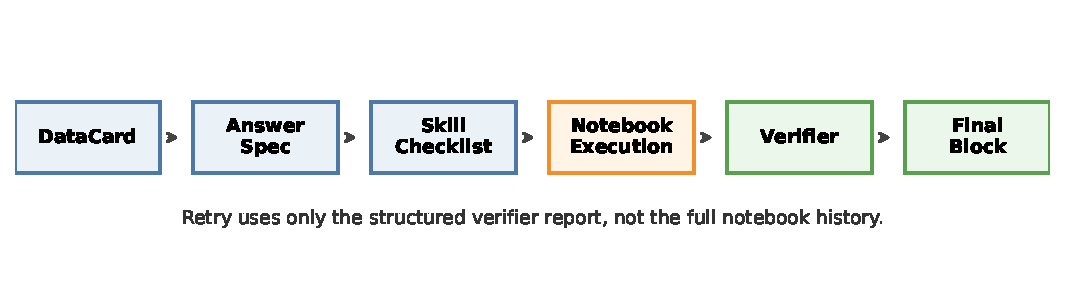
\includegraphics[width=0.9\textwidth]{artifact_pipeline}
\caption{Verifiable artifact pipeline. Each stage emits a compact artifact that can be checked before the next stage consumes it. Repair is conditioned on the structured verifier report rather than the full notebook history.}
\label{fig:artifact_pipeline}
\end{figure*}

\subsection{Lightweight vs.\ Full Verification Regimes}

We define two structured interaction regimes as configurable harness switches:

\begin{itemize}
    \item \textbf{\texttt{harness\_light}}: Enables DataCard, Answer Spec, Skill Checklist, Final Block, and programmatic formatting. Disables semantic oracle verification and multi-branch search. Suitable for low-to-medium risk questions where format constraints alone suffice to prevent the most common errors.
    \item \textbf{\texttt{harness\_full}}: Extends light with semantic oracle verification (checking statistical method correctness, preprocessing order, and output semantics), targeted retry on verification failure, and optional multi-branch execution with branch selection for hard questions.
\end{itemize}

These are not model size distinctions---the same model is used in both regimes. The difference is purely in which harness modules are active. This enables clean ablation of the marginal benefit of semantic verification over format constraints alone.

\subsection{Results}

Table~\ref{tab:structured_results} compares the two regimes against a baseline with only the original reformat mechanism (a simple post-hoc answer extraction without structural constraints). Experiments use Qwen3.5-Flash, a smaller and faster model, to stress-test whether structure can compensate for weaker reasoning capability.

\begin{table*}[t]
\centering
\caption{Structured interaction results (Qwen3.5-Flash, InfiAgentBench small-set).}
\label{tab:structured_results}
\begin{tabular}{lccc}
\toprule
\textbf{Setting} & \textbf{ABQ} & \textbf{Hard ABQ} & \textbf{Avg Runtime (s)} \\
\midrule
Baseline + original reformat & 48.94\% & 44.00\% & 30.24 \\
\texttt{harness\_light} & 51.57\% & 47.32\% & 37.03 \\
\texttt{harness\_full} & 52.83\% & 49.44\% & 43.79 \\
\bottomrule
\end{tabular}
\end{table*}

\begin{figure*}[t]
\centering
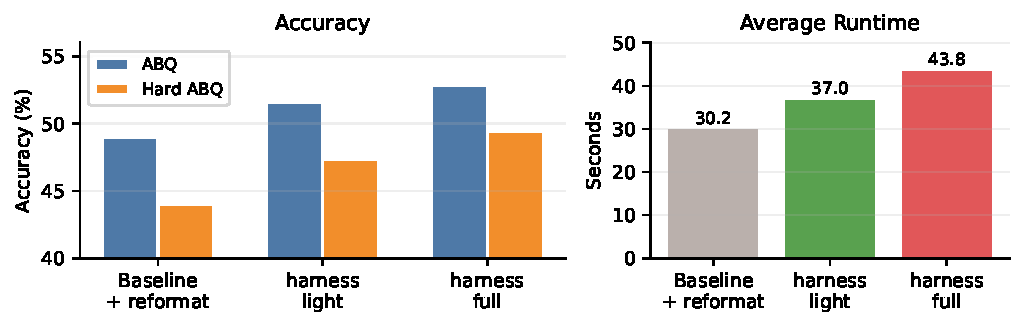
\includegraphics[width=0.86\textwidth]{structured_results}
\caption{Structured interaction on the Qwen3.5-Flash small-set experiment. Lightweight structure improves accuracy with modest overhead, while full verification provides additional gains on harder questions at higher runtime.}
\label{fig:structured_results}
\end{figure*}

Both structured regimes outperform the baseline, confirming that even lightweight constraints (DataCard + Answer Spec + Final Block) provide measurable gains over unstructured reformatting. The \texttt{harness\_light} improves ABQ by 2.63pp and Hard ABQ by 3.32pp at a modest 6.8s runtime increase. The \texttt{harness\_full} adds another 1.26pp ABQ and 2.12pp Hard ABQ at an additional 6.8s cost. Whether full verification is worthwhile depends on the task: for questions where format constraints suffice (the majority of Easy/Medium), light is the better choice; for hard questions where semantic errors are more likely, full verification provides net benefit.

These results inform our resource scheduling: the right question is not ``light or full?'' but ``which tasks need full verification, and which can succeed with light constraints?'' This risk-based dispatch is the subject of Section~\ref{sec:resource}.

\subsection{Artifact Reuse and Communication Efficiency}

An underappreciated benefit of the artifact pipeline is that verifiable artifacts serve as compact communication channels between stages. The DataCard for a given CSV is computed once and reused across all questions on that dataset, eliminating redundant data exploration. The Answer Spec compresses what would otherwise be a long natural language prompt into a structured specification. The Verifier report replaces full notebook retransmission with a short diagnostic. These savings compound: in our experiments, artifact reuse reduces the average tokens per question by approximately 30\% compared to re-reading and re-describing the dataset at each interaction turn.

\section{Resource-Aware Scheduling}
\label{sec:resource}

\subsection{The EqTok Metric}

Comparing resource consumption across heterogeneous model families requires a common unit. Raw token count is misleading because tokens from different models have different prices. API call count is also misleading because a single 32B call may cost more than several 8B calls. We define \textbf{EqTok} (Equivalent Tokens) as a pricing-weighted token count:

\begin{equation}
\mathrm{EqTok} = T_{32B} + 0.5 \cdot T_{14B} + 0.25 \cdot T_{8B}
\label{eq:eqtok}
\end{equation}

where $T_{M}$ is the total output tokens consumed by model size $M$. The coefficients reflect the Qwen API pricing ratio of approximately 1:2:4 for the 8B:14B:32B tiers on the deployment platform used in our experiments. EqTok normalizes all token consumption to 32B-equivalent units, enabling direct comparison of configurations that mix models of different sizes. The metric is provider- and family-specific: the coefficients should be recalibrated for different pricing structures.

\subsection{Risk-Stratified Sub-Task Routing}

We decompose the agent pipeline into nine sub-tasks and assign each to a processing tier based on the risk that an error at that stage will propagate to the final answer:

\begin{table*}[t]
\centering
\caption{Risk-stratified sub-task routing. Each sub-task is assigned to the lowest-cost processing tier consistent with acceptable error risk.}
\label{tab:risk_routing}
\footnotesize
\begin{tabular}{p{0.22\textwidth}p{0.38\textwidth}p{0.28\textwidth}}
\toprule
\textbf{Sub-Task} & \textbf{Description} & \textbf{Tier} \\
\midrule
Data Profiling & Read schema, types, missing values, ranges & Deterministic \\
Answer Spec Parsing & Extract answer name, columns, format & Rule-first; 8B/14B fallback \\
Task Routing & Classify concept, difficulty, risk level & Rule-first; 8B/14B fallback \\
Step Planning & Decompose question into analysis steps & 8B (easy), 14B (med), 32B (hard) \\
Code Generation & Write data processing / ML code & 14B (easy), 32B (med/hard) \\
Debugging & Fix runtime and logic errors & 8B/14B (simple), 32B (complex) \\
Post-Debug Cleanup & Remove error cells, keep working path & Deterministic \\
Verification & Check constraints against Answer Spec & Deterministic \\
Final Formatting & Render into required output format & Deterministic \\
\bottomrule
\end{tabular}
\end{table*}

The key principle is risk-proportional resource allocation: deterministic sub-tasks (data profiling, verification, formatting, cleanup) never trigger an LLM call. For LLM-dependent sub-tasks, model size is chosen by the estimated difficulty of that specific sub-task rather than by a global setting. Easy step planning uses an 8B model; hard code generation uses a 32B model. This differs from the common default of using the same model for every sub-task regardless of difficulty.

\subsection{Dialogue Reduction Mechanisms}

Beyond model routing, we reduce total LLM calls through five complementary mechanisms:

\begin{enumerate}
    \item \textbf{Deterministic Artifacts}: DataCard, Answer Spec parsing (when unambiguous), and Final Block are computed deterministically, avoiding repeated model queries for tasks with well-defined answers.
    \item \textbf{Spec-to-Plan Generation}: Structured Answer Specs directly generate operation plans through template expansion, reducing the free-form exploration that consumes tokens without producing useful output.
    \item \textbf{One-Shot Execution}: Low-risk questions (Simple Statistics on Easy difficulty) are completed in a single model call with pre-filled DataCard and Answer Spec, avoiding the multi-turn planning overhead.
    \item \textbf{Verifier-Triggered Retry}: Only verification failures trigger repair, and the repair input is the structured failure report, not the full conversation history.
    \item \textbf{Cross-Question Artifact Reuse}: Data profiling results and column normalizations are cached and reused across questions sharing the same dataset, eliminating redundant data exploration calls.
\end{enumerate}

\subsection{Resource Ablation Results}

Table~\ref{tab:resource_results} presents the resource ablation study. Three configurations are compared: (1) the 32B baseline using a single large model for all stages; (2) ``Small Model Rules,'' which routes deterministic sub-tasks to rules and uses smaller models for low-risk stages; and (3) ``+ Dialogue Reduction,'' which additionally enables the five mechanisms described above.

\begin{table*}[t]
\centering
\caption{Resource ablation results on InfiAgentBench. EqTok is reported in millions of 32B-equivalent tokens.}
\label{tab:resource_results}
\begin{tabular}{lccc}
\toprule
\textbf{Configuration} & \textbf{ABQ} & \textbf{EqTok (M)} & \textbf{API Calls} \\
\midrule
32B baseline & 81.74\% & 5.960 & 1,621 \\
Small Model Rules & 78.42\% & 3.517 & 1,956 \\
+ Dialogue Reduction & 78.63\% & 3.298 & 1,874 \\
\bottomrule
\end{tabular}
\end{table*}

\begin{figure*}[t]
\centering
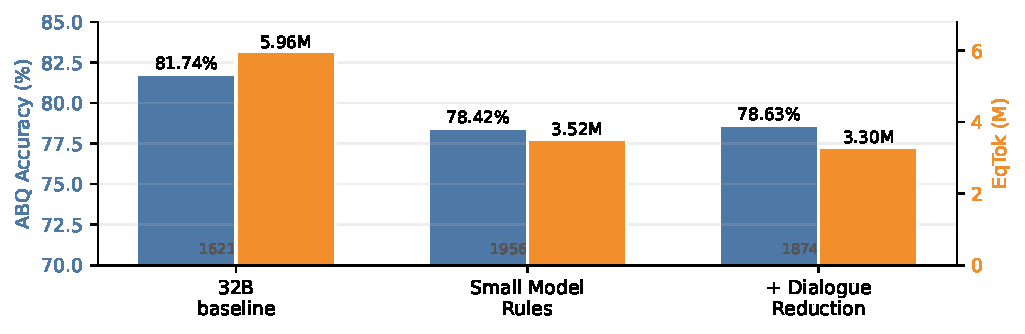
\includegraphics[width=0.86\textwidth]{resource_ablation}
\caption{Resource ablation with pricing-normalized EqTok. Smaller-model routing increases the number of API calls but sharply reduces 32B-equivalent token cost, retaining most of the baseline ABQ accuracy.}
\label{fig:resource_ablation}
\end{figure*}

The Small Model Rules configuration reduces EqTok by 41.0\% (from 5.96M to 3.52M) while retaining 95.9\% of baseline accuracy (78.42\% vs.\ 81.74\%). Dialogue reduction further decreases EqTok to 3.30M (44.7\% total savings) with a marginal accuracy gain (78.63\%), confirming that eliminating redundant model calls does not hurt and may help by reducing context noise.

Notably, the resource-efficient configurations exhibit higher API call counts (1,956 and 1,874 vs.\ 1,621) despite lower total resource consumption. This reflects a fundamental trade-off: smaller models require more debugging rounds because they make more frequent errors, but each round is substantially cheaper. The EqTok metric correctly captures this trade-off where raw call count would misleadingly suggest the resource-efficient configuration is more expensive.

These results validate a central claim: resource optimization is not about replacing large models entirely, but about reserving them for sub-tasks where reasoning depth genuinely matters. Strong models are not necessarily slower (they may require fewer rounds), and small models are not necessarily cheaper (they may require more rounds). The right metric is EqTok integrated over the full pipeline, and the right strategy is risk-stratified routing.

\section{Integrated Architecture}
\label{sec:integration}

Figure~\ref{fig:architecture} illustrates the integrated DatawiseAgent architecture that unifies our three contributions. The pipeline proceeds from question ingestion through task routing, answer specification, memory filtering, risk estimation, execution, validation, and final submission. Each stage's processing tier is determined by the risk estimator based on question difficulty, concept complexity, and verification history from prior questions.

\begin{figure*}[t]
\centering
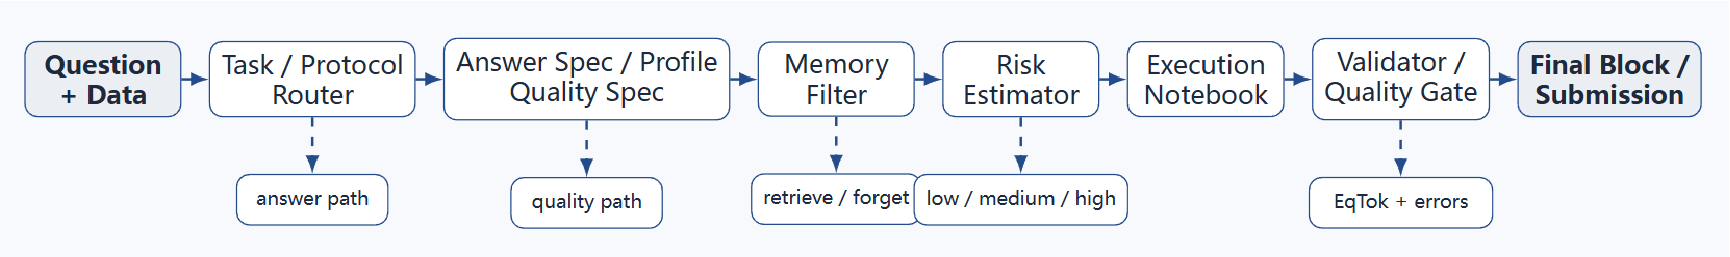
\includegraphics[width=0.9\textwidth]{fig1}
\caption{Integrated Resource-Aware DatawiseAgent architecture. The pipeline proceeds from question ingestion through task routing, answer specification, memory filtering, risk estimation, notebook execution, validation, and final submission. Each stage's processing tier is determined by the risk estimator based on question difficulty, concept complexity, and verification history.}
\label{fig:architecture}
\end{figure*}

The integrated design yields three operational principles that synthesize findings across all three contribution areas:

\begin{enumerate}
    \item \textbf{Failure modes are not uniform}: InfiAgentBench errors stem from answer definition, statistical rules, and output format; DataModeling errors stem from submission quality, metrics, manifests, and low-information predictions. The harness must be task-specific rather than monolithic.
    \item \textbf{Completion $\neq$ Performance}: Qwen3-VL achieves 74/74 structural completion on DataModeling but low predictive performance (0.29--0.31). A Quality Gate that detects degenerate predictions is essential, but cannot fix them---closing this gap requires model-level improvement.
    \item \textbf{Memory and harness both need selectivity}: Full memory retention degrades retrieval signal-to-noise ratio; full harness can overburden weak models. The key is retaining only high-value, high-recency context and applying constraints proportional to risk.
\end{enumerate}

\section{Discussion and Boundary Analysis}
\label{sec:discussion}

\subsection{When Training-Free Harness Improvements Are Insufficient}

Our results also reveal boundary conditions where harness engineering cannot substitute for model capability:

\begin{itemize}
    \item \textbf{Multi-Concept Hard Questions}: All 19 Machine Learning questions in InfiAgentBench are classified as Hard and combine ML with Comprehensive Preprocessing or Feature Engineering. These questions require simultaneous reasoning about feature engineering, model selection, hyperparameter tuning, and validation strategy. No amount of format constraint can fix fundamentally incorrect modeling choices---the harness can ensure the answer is well-formed, but not that it is correct.
    \item \textbf{DataModeling Performance Gap}: While the strong model achieves 73/74 completion, the normalized performance score of 0.5318 indicates substantial room for improvement. Low-score patterns include multi-class collapse (predicting a single class), text data misrouting (applying tabular methods to NLP tasks), and time-series/grouped tasks treated as ordinary tables. These require domain-specific modeling strategies beyond generic harness constraints.
    \item \textbf{Memory Saturation}: Our preliminary memory experiments (tracking retrieval quality over interaction history length) show that storing all history causes retrieval signal-to-noise ratio to degrade over time, consistent with theoretical expectations. A selective forgetting mechanism based on artifact importance and recency is needed, with the forgetting curve calibrated to maintain retrieval quality without discarding useful context.
\end{itemize}

\subsection{Design Principles for Resource-Aware Data Science Agents}

From our experimental findings, we distill five design principles:

\begin{enumerate}
    \item \textbf{Classify before constraining}: Route questions to protocol-specific harnesses based on concept taxonomy rather than applying uniform constraints. Summary Statistics needs strict numerical constraints; Machine Learning needs model documentation requirements; Correlation needs method declaration.
    \item \textbf{Verify at artifact boundaries}: Check each stage's output before passing it to the next stage. When verification fails, retry with the failure report only, not the full history. This keeps contexts short and focused.
    \item \textbf{Match model size to risk}: Use deterministic programs for no-risk stages (profiling, formatting), small instruct models for low-risk reasoning (simple planning, easy debugging), and large models only for high-risk code generation and complex debugging.
    \item \textbf{Measure holistically with EqTok}: Evaluate resource efficiency in pricing-equivalent tokens rather than raw token count or API call count alone. Raw counts produce misleading comparisons when model sizes are heterogeneous.
    \item \textbf{Accept training-free limits}: Harness engineering improves the probability of correct execution but cannot guarantee correct reasoning. For the hardest tasks, model capability remains the binding constraint, and hybrid approaches combining harness optimization with fine-tuning or stronger base models are needed.
\end{enumerate}

\subsection{Limitations and Future Work}

Our study has several limitations that motivate future work. \textbf{First}, our resource ablation covers only the Qwen model family; the EqTok coefficients would differ for other providers, and the risk-stratified routing table may need recalibration for models with different capability gaps between size tiers. \textbf{Second}, the task router currently relies on benchmark metadata for difficulty labels and concept annotations; fully automatic difficulty estimation from question text alone, perhaps via embedding-based classification, remains an open challenge for production deployment. \textbf{Third}, our memory experiments are preliminary and do not yet include a production-quality forgetting mechanism with calibrated importance and recency thresholds. \textbf{Fourth}, the DataModeling Quality Gate can detect degenerate predictions (constant outputs, single-class collapse) but cannot fix them---closing the completion-to-performance gap requires either model-level improvements, domain-specific fine-tuning, or more sophisticated repair strategies.

Future work includes: (1) extending the risk-stratified scheduler to additional model families (e.g., GPT, Claude, Gemini) and calibrating family-specific EqTok coefficients; (2) developing automatic difficulty estimators based on question embeddings and historical performance patterns; (3) implementing artifact-importance-based memory pruning with empirically calibrated forgetting curves; (4) exploring fine-tuning strategies that specifically target the failure modes identified in this study (answer-name matching, statistical definition stabilization, format compliance); and (5) investigating whether the three-part optimization framework generalizes to other agent domains beyond data science, such as code generation or scientific reasoning.

\section{Conclusion}

We presented a systematic study of three interconnected challenges in deploying LLM-based data science agents: task-specific failure heterogeneity that generic harnesses cannot address, the non-monotonic value of long unstructured interactions, and high resource consumption from uniform large-model deployment. Through DatawiseAgent, we showed that (1) a task-aware harness with protocol routing eliminates format-level errors and improves accuracy by 8--12 percentage points on InfiAgentBench; (2) structuring long interactions into verifiable artifacts with targeted, failure-report-only retry reduces context contamination and improves weak-model performance; and (3) risk-stratified scheduling with the EqTok metric achieves approximately 40\% resource savings while maintaining 96\% of baseline accuracy. Our boundary analysis clarifies where training-free engineering reaches its limits: hard multi-concept questions, low-information predictive submissions, and memory saturation. The resulting design principles---classify before constraining, verify at artifact boundaries, match model size to risk, measure holistically with EqTok, and accept training-free limits---offer actionable guidance for building cost-effective and reliable data science agents.

\bibliography{datawiseagent_refs}

\end{document}
